\documentclass[border=0.5mm]{standalone}
\usepackage{tikzducks,tikzlings}
\usepackage{worldflags}
\begin{document}

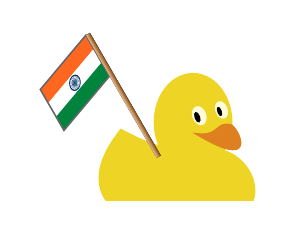
\begin{tikzpicture}%[xscale=-1]
 \clip (-1.2,-1.5) rectangle ++ (3,2.2);

 \begin{scope}[xscale=-1,xshift=-1.8cm,yshift=-2cm]
  \duck
\end{scope}  

\begin{scope}[x=0.3mm,y=0.3mm,xscale=1]
\pgfdeclarehorizontalshading{flagpole}
{30mm}{color(0mm)=(white);
color(1mm)=(brown); color(2mm)=(black)}
\flagsdefault[width=6mm,hang=20]
\pic (in) [country=IN,rotate=30,turn=180]
at (-20,0) {worldflag};
\fill [shading=flagpole,shading angle=30,
rotate around={30:(in-nw)}]
(in-nw)-|++(2,-60)-|cycle;
\end{scope}

\end{tikzpicture}

\end{document} 